\documentclass[a4paper,8pt]{report}

\usepackage[francais]{babel}
\usepackage[T1]{fontenc}
\usepackage[utf8]{inputenc}

\usepackage[left=2cm]{geometry}
\usepackage{amsmath,amssymb,mathrsfs}
\usepackage{graphicx}
\usepackage[table,xcdraw]{xcolor}

%Utilisation des codes sources en C
\usepackage{listings}
\lstset{
  language=C,
  language=Bash,
  basicstyle=\footnotesize,
  numbers=left,
  numberstyle=\normalsize,
  numbersep=7pt,
}

%titre pdf
\title{{\LARGE Algorithmique Avanc\'ee \\ Devoir de Programmation : Tries}}
\author{ilyas Toumlilt - 3261538\\Mohamed Amin Affes - 3262731}

\graphicspath{{graph/}}

\begin{document}

\maketitle
\renewcommand{\contentsname}{Sommaire}
\tableofcontents

%%%%%%%%%%%%%%%%%%%%%%%%%%%%%%%%%%%%%%%%%%%%%%%%%%%%%%%%%%%%%%%%%%%%%%%%%%%%%%%%%%%%%%%%%%%%%%%%%%%%%%%%%%%%%
% Présentation
%%%%%%%%%%%%%%%%%%%%%%%%%%%%%%%%%%%%%%%%%%%%%%%%%%%%%%%%%%%%%%%%%%%%%%%%%%%%%%%%%%%%%%%%%%%%%%%%%%%%%%%%%%%%%
\chapter{Pr\'esentation}

\section*{Introduction}\label{sec:name}
\addcontentsline{toc}{section}{Introduction}
\textit{``Le but du probl\`eme consiste \`a repr\'esenter un dictionnaire de mots. Dans cette optique, nous proposons l'implementation de deux structures de tries concurrentes puis une \'etude exp\'erimentale permettant de mettre en avant les avantages et inconv\'enients de chacun des mod\`eles. En plus des implantations des structures des donn\'ees et des primitives de base, nous envisageons une fonction avanc\'ee pour chancun des mod\`eles.''}\\
Les structures utilisées sont les arbres de la Briandais et les tries Hybrides.

\section*{Conception}\label{sec:name}
\addcontentsline{toc}{section}{Conception}
Pour pouvoir travailler en concurrence, la réalisation du projet a été divisée en deux parties, chaque binôme s'occupe donc de l'implémentation de l'une des deux structures.\\
D'un point de vue programmatique, chaque composant de structure (noeud, arbre, liste, vues .. ) a été implémenté comme une librairie indépendante contenant ses propres primitives, ce qui facilite leur importation et assure une utilisation indépendante.\\

\section*{Le langage C : pourquoi ?}\label{sec:name}
\addcontentsline{toc}{section}{Le langage C : pourquoi ?}
Le choix du langage de programmation s'est porté sur le C, vu les facilitées qu'il apporte à la gestion des structures de données ainsi qu'au niveau du contrôle de la mémoire, ainsi nous fournissons dans chaque librairie des fonctions permettant la libération de la mémoire, et nous garantissons que les programmes de test se terminent avec 0 octets dans la mémoire.

\section*{Organisation}\label{sec:name}
\addcontentsline{toc}{section}{Organisation}
Les sources du projet sont contenus dans le répertoire sources/.
Ainsi à chaque fois qu'on donnera un pointeur vers un fichier, il aura comme racine ce dossier.

%%%%%%%%%%%%%%%%%%%%%%%%%%%%%%%%%%%%%%%%%%%%%%%%%%%%%%%%%%%%%%%%%%%%%%%%%%%%%%%%%%%%%%%%%%%%%%%%%%%%%%%%%%%%%
% Structures
%%%%%%%%%%%%%%%%%%%%%%%%%%%%%%%%%%%%%%%%%%%%%%%%%%%%%%%%%%%%%%%%%%%%%%%%%%%%%%%%%%%%%%%%%%%%%%%%%%%%%%%%%%%%%
\chapter{Structures}

\section*{Structure 1 : Arbres de la Briandais}\label{sec:name}
\addcontentsline{toc}{section}{Structure 1 : Arbres de la Briandais}
Parmi les 128 caractères du code ASCII, on considère '$\backslash$0' comme marqueur de fin de mot, ce qui offre des facilitées de programmation vu que c'est le premier caractère dans l'ordre ASCII. Ce caractère est défini dans la globale ASCII\_EOW dans include/libASCII.h et permet sa modification si on le souhaite.\\
Tous les fichiers et toutes les fonctions de la librairie sont préfixés BRD.\\
Structure et primitives d'un noeud BRD ( include/BRDnode.h ):
\begin{verbatim}
  typedef struct _BRDnode {
    char content;                 /* contenu du noeud */
    struct _BRDnode* firstChild;  /* branche vers fils */
    struct _BRDnode* nextSibling; /* branche vers le frère */ 
  } BRDnode;
  BRDnode* BRDinitNodeWithValue(char value);
  --> Alloue et retourne un nouveau noeud initialisé à value.
  BRDnode* BRDinitEmptyNode();
  --> Alloue et retourne un nouveau noeud initialisé à ASCII_EOW
  BRD[get/set][Content/FirstChild/NextSibling]
  --> accesseurs des valeurs de la structure
  BRDisEmptyNode(BRDnode* node);
  --> Test si le noeud est vide ou pas.
  BRDhas[FirstChild/NextSibling](BRDnode* node);
  --> Test si le noeud contient un (Fils/Frère)
  BRDfreeNode(BRDnode* node);
  --> désalloue la mémoire du noeud.
\end{verbatim}
Structure est primitives d'un arbre BRD ( include/BRDtree.h ) :
\begin{verbatim}
  typedef struct _BRDtree {
    BRDnode* topOfTree; /* Sommet de l'arbre */
  } BRDtree;
  BRDtree* BRDinitTreeWithNode(BRDnode* node);
  --> Alloue et retourne un nouvel arbre initialisé à node
  BRDtree* BRDinitEmptyTree();
  --> Alloue et retourne un arbre vide
  BRD[get/set]TopOfTree(BRDtree* tree);
  --> accesseurs du sommet de l'arbre.
  BRDfreeTree(BRDtree* tree);
  --> Désalloue un arbre
\end{verbatim}

\section*{Structure 2 : Tries Hybrides}\label{sec:name}
\addcontentsline{toc}{section}{Structure 2 : Tries Hybrides}
Tous les fichiers et toutes les fonctions de la librairie sont préfixés TRH.\\
Structure et primitives d'un noeud TRH ( include/TRHnode ) :
\begin{verbatim}
  typedef struct _TRHnode {
    char content; /* caractère représenté par le noeud */
    int keyValue; /* non vide ( != -1 ) lorsque le noeud est une clé */
    int id; /* unique par noeud, pour la représentation graphique */
    struct _TRHnode *lowChild;
    struct _TRHnode *equalChild;
    struct _TRHnode *highChild;
  } TRHnode;
  TRHnode* TRHinitNodeWithContent(char content);
  --> Allocation d'un noeud avec contenu
  void TRHfreeNode(TRHnode* node);
  --> Désalloue un noeud
  TRH[set/get]<composant>
  --> Accesseurs
  int TRHisEmptyNode(TRHnode* node);
  --> test si le noeud et vide
\end{verbatim}
Strucuture est primitives d'un arbre TRH ( include/TRHtree.h ) :
\begin{verbatim}
  typedef struct _TRHtree {
    TRHnode* topOfTree;
  } TRHtree;
  TRHtree* TRHinitEmptyTree();
  --> Alloue un arbre vide.
  void TRHfreeTree(TRHtree* tree);
  --> Désallocation d'un arbre.
  TRH[get/set]TopOfTree
  --> Accesseurs
  int TRHisEmptyTree(TRHtree* tree);
  --> Test si l'arbre est vide
\end{verbatim}

%%%%%%%%%%%%%%%%%%%%%%%%%%%%%%%%%%%%%%%%%%%%%%%%%%%%%%%%%%%%%%%%%%%%%%%%%%%%%%%%%%%%%%%%%%%%%%%%%%%%%%%%%%%%%
% Fonctions avancées 
%%%%%%%%%%%%%%%%%%%%%%%%%%%%%%%%%%%%%%%%%%%%%%%%%%%%%%%%%%%%%%%%%%%%%%%%%%%%%%%%%%%%%%%%%%%%%%%%%%%%%%%%%%%%%
\chapter{Fonctions avancées pour chacune des structures}

\section*{Arbres de la Briandais}\label{sec:name}
\addcontentsline{toc}{section}{Arbres de la Birandais}
Toutes les fontions avancées sont définies dans l'API de librairies BRD : include/BRD\_API.h\\ \\
%Recherche :
Fonction de recherche d'un mot dans le dictionnaire :
\begin{verbatim}
  int BRDsearchWord(BRDtree* tree, char* word, int size); <src/BRD_API.c>
  --> cherche un mot dans l'arbre.
  --> Principe : on parcours les caractères du mot, et pour chacun on cherche le noeud
                 contenant ce caractère dans le niveau actuel ( liste des frères ), une
                 fois trouvé, on passe au caractère suivant et on le cherche dans la 
                 liste du fils du noeud précédemment trouvé. Si on ne trouve pas le 
                 caractère dans le niveau, on renvoie Faux ( 0 ).
\end{verbatim}
%ComptageMots :
Fonction qui compte le nombre de mots présents dans le dictionnaire :
\begin{verbatim}
  int BRDcountTreeWords(BRDtree* tree); <src/BRD_API.c>
  --> Test si l'arbre n'est pas vide, puis fait appel à la fonction auxiliaire :
  int BRDcountWordsFromNode(BRDnode* node); <src/BRD_API.>
  --> Principe : On parcours récursivement tous les noeuds de l'arbre, puis à chaque
                 noeud contenant le caractère de fin de mot, on incrémente le compteur.
\end{verbatim}
%ListMots
Fonction qui liste les mots du dictionnaire dans l'ordre alphabétique :
\begin{verbatim}
  ListWord* BRDgetListWordFromTree(BRDtree* tree); <src/BRD_API.c>
  --> Test si l'arbre n'est pas vide, puis fait appel à la fonction auxiliaire :
  ListWord* BRDinitListWordFromNode(BRDnode* node, ListWord** end, char* word, int size);
  --> Principe : Cette fonction récursive permet de récupéré le début de la liste créée 
                 et sa fin ( dans end ), on passe également à chaque fosi le préfixe du mot
                 constitué jusqu'à présent et sa taille, on rajoute le char en cours à 
                 chaque appel et on l'enlève à chaque retour.
                 Pour chaque noeud, s'il contient un fils, on fait un appel récursif sur
                 ce dernier, sinon s'il est un char de fin de mot, on initialise un element
                 de la liste avec le mot courant, puis s'il a un next sibling, on fait un
                 appel récursif sur ce dernier.
                 A la fin, on rassemble les listes créée en rajoutant celle des frères
                 à la suite de celle des fils ( vu qu'on récupère le dernier elem )
\end{verbatim}
%ComptageNil :
Fonction qui compte les pointeurs vers Nil
\begin{verbatim}
  int BRDcountTreeNullNodes(BRDtree* tree); <src/BRD_API.c>
  --> Test si l'arbre n'est pas vide, puis fait appel à la fonction auxiliaire :
  int BRDcountNullNodesFromNode(BRDnode* node); <src/BRD_API.c>
  --> Principe : Cette fonction récursive fait deux tests à chaque fois :
                 - si le fils est NULL elle incrémente le compteur sinon elle se
                   relance dessus.
                 - si le frère est NULL elle incrémente le compteur sinon elle se
                   relance dessus.
\end{verbatim}
%Hauteur :
Fonction qui calcule la hauteur de l'arbre
\begin{verbatim}
  int BRDcountTreeHeight(BRDtree* tree); <src/BRD_API.c>
  --> Test si l'arbre n'est pas vide, puis fait appel à la fonction auxiliaire :
  int BRDcountHeightFromNode(BRDnode* node); <src/BRD_API.c>
  --> Principe : Cette fonction récursive fait :
                 - si le fils est vide retourne 1 si le frère est vide, ou le résultat
                   de l'appel récursif sur le frère sinon
                 - si le fils n'est pas vide retourne le Max entre l'appel récursif sur
                   le fils + 1 et l'appel récursif sur le frère.
\end{verbatim}
%ProfondeurMoyenne
Fonction qui calcule la profondeur moyenne des feuilles de l'arbre
\begin{verbatim}
  int BRDcountAverageDepth(BRDtree* tree); <src/BRD_API.c>
  --> Test si l'arbre n'est pas vide, puis fait appel à la fonction auxiliaire :
  void BRDcountAverageDepthFromNode(BRDnode* node, AverageDepth** ad, int h); <src/BRD_API.c>
  --> Principe : Utilise la struct de la librairie AverageDepth
                 <include/AverageDepth.h>, fait un parcours complet de l'arbre, puis
                 à chaque noeud incrémente le nombre de noeuds dans la struct
                 et à chaque fin rajoute la hauteur.
                 A la fin de la récursivité ( retour au sommet ), on calcule
                 la profondeur en faisant la division puis on renvoie le résultat
\end{verbatim}
%Prefixe
Fonction qui calcule le nombre de mots préfixés par un mot A passé en argument
\begin{verbatim}
  int BRDcountTreePrefixeOccurrence(BRDtree* tree, char* word, int size); <src/BRD_API.c>
  --> Principe : Parcours le mot, puis pour chaque caractère cherche le noeud
                 le noeud le contenant dans le niveau actuel, si trouvé on passe
                 au niveau et au caractère suivant sinon on renvoie 0.
                 Après recherche de tous les caractères du préfixe, on lance
                 un comptage de mots à partir de ce noeud ( fonction présentée 
                 précédemment ).
\end{verbatim}
%Suppression
Fonction qui supprime un mot de l'arbre
\begin{verbatim}
  int BRDremoveWordFromTree(BRDtree* tree, char* word, int size); <src/BRD_API.c>
  --> Principe : Le traitement se compose de deux étapes :
                 - D'abord on fait un parcours du mot lettre par lettre et de
                   l'arbre niveau en cherchant à chaque fois le bon noeud
                   comme pour le prefixe, sauf que cette fois, à chaque noeud
                   trouvé, on mettra son adresse dans un tableau de d'adresses
                   de noeuds. Cette première étape permettra de récupérer les
                   adresses de tous les noeuds à supprimer ainsi que vérifier
                   l'existance du mot.
                 - Ensuite on va parcourir le tableau d'adresses ( du bas vers
                   le haut ), en prenant soin de garder le bon état de l'arbre :
                 -- Si c'est un premier fils qu'on supprime, le père doit pointer
                    sur son suivant
                 -- Sinon son frère gauche doit pointer sur son droit.
                 -- S'il a encore des fils, on ne le supprime pas.
\end{verbatim}

\section*{Tries Hybrides}\label{sec:name}
\addcontentsline{toc}{section}{Tries Hybrides}
Toutes les fontions avancées sont définies dans l'API de librairies TRH : include/TRH\_API.h\\ \\
%Recherche :
Fonction de recherche d'un mot dans le dictionnaire :
\begin{verbatim}
  int TRHsearchWord(TRHtree* tree, char* word, int size); <src/TRH_API.c>
  --> Test si l'arbre n'est pas vide puis fait appel à la fonction auxiliaire :
  int TRHsearchwordFromNodeRecursive(TRHnode* node, char* word, int size); <TRH_API.c>
  --> Principe : Pour chaque noeud :
                 - S'il est égale à word[0] :
                 -- si size == 1 est que c'est une fin de mot : on renvoie TRUE
                 -- si size == 1 est que ce n'est pas une fin de mot : FALSE
                 -- si size != 1 appel récursif sur le fils égal avec word+1
                    et size-1
                 - s'il est inférieur à word[0] : appel récursif sur le fils
                   gauche s'il existe
                 - s'il est supérieur à word[0] : appel récursif sur le fils
                   droit s'il existe
                 - sinon : retourne FALSE
\end{verbatim}
%ComptageMots :
Fonction qui compte le nombre de mots présents dans le dictionnaire :
\begin{verbatim}
  int TRHcountWords(TRHtree* tree); <src/TRH_API.c>
  --> Test si l'arbre n'est pas vide, puis fait appel à la fonction auxiliaire :
  int TRHcountWordsFromNodeRecursive(TRHnode* node); <src/TRH_API.>
  --> Principe : Fonction récursive, fait un parcours de tout l'arbre, à chaque
                 Noeud de fin de mot, renvoie 1 + appels récursifs sur les fils
                 existes.
\end{verbatim}
%ListMots
Fonction qui liste les mots du dictionnaire dans l'ordre alphabétique :
\begin{verbatim}
  ListWord* TRHinitListWordFromTree(TRHtree* tree); <src/TRH_API.c>
  --> Test si l'arbre n'est pas vide, puis fait appel à la fonction auxiliaire :
  ListWord* TRHinitListWordFromNode(TRHnode* node, ListWord** end, char* word, int size);
  --> Principe : Cette fonction récursive permet de récupérer le début et la fin
                 de la liste créée à chaque fois, le début est retourné et
                 l'adresse de la fin est mise dans le param end.
                 Fait d'abord un appel récursif sur le fils gauche s'il existe,
                 puis rajoute à sa fin le mot actuel si on est en fin de mot,
                 puis le résultat de l'appel récursif sur le fils égal s'il
                 existe, à qui on rajoute le résultat de l'appel récursif
                 sur le fils droit s'il existe.
                 Le mot construit jusqu'à présent et passé dans le param
                 word ainsi que sa taille.
\end{verbatim}
%ComptageNil :
Fonction qui compte les pointeurs vers Nil
\begin{verbatim}
  int TRHcountNil(TRHtree* tree); <src/TRH_API.c>
  --> Test si l'arbre n'est pas vide, puis fait appel à la fonction auxiliaire :
  int TRHcountNilFromNodeRecursive(TRHnode* node); <src/TRH_API.c>
  --> Principe : Cette fonction est récursive, et pour chaque noeud, va
                 faire un test d'existence pour chaque fils :
                 - s'il est NULL : compteur + 1
                 - sinon : compteur + résultat appel récursif sur ce fils
\end{verbatim}
%Hauteur :
Fonction qui calcule la hauteur de l'arbre
\begin{verbatim}
  int TRHcountHeight(TRHtree* tree); <src/TRH_API.c>
  --> Test si l'arbre n'est pas vide, puis fait appel à la fonction auxiliaire :
  int TRHcountHeightFromNodeRecursive(TRHnode* node); <src/TRH_API.c>
  --> Principe : Cette fonction récursive retourne 1 + le max des trois
                 appels récursifs vers les fils s'ils existent.
\end{verbatim}
%ProfondeurMoyenne
Fonction qui calcule la profondeur moyenne des feuilles de l'arbre
\begin{verbatim}
  int TRHcountAverageDepth(TRHtree* tree); <src/TRH_API.c>
  --> Test si l'arbre n'est pas vide, puis fait appel à la fonction auxiliaire :
  void TRHcountAverageDepthFromNode(TRHnode* node, AverageDepth** ad, int h); <src/TRH_API.c>
  --> Principe : Utilise la struct de la librairie AverageDepth
                 <include/AverageDepth.h>, fait un parcours complet de l'arbre, puis
                 à chaque noeud incrémente le nombre de noeuds dans la struct
                 et à chaque fin rajoute la hauteur.
                 A la fin de la récursivité ( retour au sommet ), on calcule
                 la profondeur en faisant la division puis on renvoie le résultat
\end{verbatim}
%Prefixe
Fonction qui calcule le nombre de mots préfixés par un mot A passé en argument
\begin{verbatim}
  int BRDcountTreePrefixeOccurrence(BRDtree* tree, char* word, int size); <src/BRD_API.c>
  --> Principe : Fait un premier parcours comme dans la fonction de recherche
                 pour chercher le mot préfixe ( retourne 0 si pas trouvé )
                 puis fait un appel à la fonction de recherche de fin de mots
                 à partir de ce noeud là.
\end{verbatim}
%Suppression
Fonction qui supprime un mot de l'arbre
\begin{verbatim}
  int TRHremoveWordFromTree(TRHtree* tree, char* word, int size); <src/TRH_API.c>
  --> Principe : Le traitement se compose de deux étapes :
                 - On construit d'abord un tableau de pointeurs vers les noeuds
                   du mot à supprimer, ce parcours nous permet d'être sur que
                   le mot existe
                 - Puis on parcours notre sutructure de pointeurs en supprimant
                   ( dans le cas de fin de mots ), et en réequilibrant.
\end{verbatim}

%%%%%%%%%%%%%%%%%%%%%%%%%%%%%%%%%%%%%%%%%%%%%%%%%%%%%%%%%%%%%%%%%%%%%%%%%%%%%%%%%%%%%%%%%%%%%%%%%%%%%%%%%%%%%
% Fonctions complexes
%%%%%%%%%%%%%%%%%%%%%%%%%%%%%%%%%%%%%%%%%%%%%%%%%%%%%%%%%%%%%%%%%%%%%%%%%%%%%%%%%%%%%%%%%%%%%%%%%%%%%%%%%%%%%
\chapter{Fonctions complexes}

\section*{Fusion de deux BRD}\label{sec:name}
\addcontentsline{toc}{section}{Fusion de deux BRD}

\begin{verbatim}
  BRDtree* BRDmergeTwoTrees(BRDtree* tree1, BRDtree* tree2); <src/BRD_API.c>
  --> Fait simplement appel à la fonction auxiliaire, avec la tête des arbres :
  BRDnode* BRDmergeTwoNodesRecursive(BRDnode* n1, BRDnode* n2); <src/BRD_API.c>
  --> Principe : Fonction récursive, on fait un parcours parallèle des deux
                 des deux arbres, et à chaque noeud :
                 - si les contenus sont égaux, on rajoute à l'arbre un noeud
                   du même contenu, dont le fils et le résultat de l'appel 
                   récursif sur les fils des deux noeuds, et le frère et le
                   résultat de l'appel récursif sur les deux frères également.
                 - sinon, on rajoute celui dont le contenu est inférieur avec 
                   tous ses fils, puis le frère sera l'appel récursif avec le
                   grand noeud et le frère du petit.
\end{verbatim}

\section*{Conversions}\label{sec:name}
\addcontentsline{toc}{section}{Conversions}

Les conversions dans les deux sens fonctionnent par parcours avec construction de mot, et à chaque noeud de fin de mot, on appelle la fonction de l'autre structure qui rajoute un mot dans l'arbre.

\section*{Equilibrage d'un TRH}\label{sec:name}
\addcontentsline{toc}{section}{Equilibrage d'un TRH}

Le seuil de déséquilibre d'un trie Hybride pourrait être en fonction de la profondeur moyenne.\\
L'idée du réequilibrage est de faire la bonne rotation selon l'état de l'arbre ( facteur : profondeur moyenne ).\\
Les rotations implémentée ici sont ZIG-ZIG, ZIG-ZAG, ZAG-ZIG :
\begin{figure}[H]
  \centering
  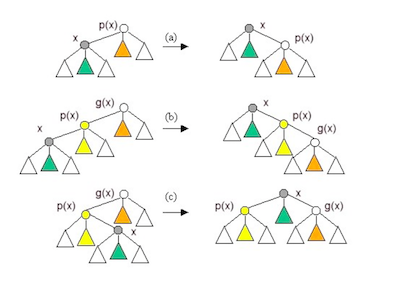
\includegraphics[width=0.8\textwidth]{rotations.png}
  \caption{Schema rotations}
  \label{fig:Schama rotations}
\end{figure}

%%%%%%%%%%%%%%%%%%%%%%%%%%%%%%%%%%%%%%%%%%%%%%%%%%%%%%%%%%%%%%%%%%%%%%%%%%%%%%%%%%%%%%%%%%%%%%%%%%%%%%%%%%%%%
% Compléxités
%%%%%%%%%%%%%%%%%%%%%%%%%%%%%%%%%%%%%%%%%%%%%%%%%%%%%%%%%%%%%%%%%%%%%%%%%%%%%%%%%%%%%%%%%%%%%%%%%%%%%%%%%%%%%
\chapter{Complexités}

\section*{Arbres de la Briandais}\label{sec:name}

\textit{fonction de recherche d'un mot dans un arbre de la Briandais}, dans le pire cas on parcours L caract\`eres (L correspond \`a la longueur du mot) donc notre complexit\'e est en O(L).\\

\smallskip
\textit{fonction de comptage de mots}, on parcours tous l'arbre (dans le pire et le meilleur cas) soit L caract\`eres et pour chaque L on parcours sa hauteur soit ln N donc notre complexit\'e est en O(L * ln N).\\

\smallskip
\textit{fonction liste de mots}, on parcours simplement tous l'arbre donc comme pour le comptage de mots nous avons une complexit\'e en O(L * ln N).\\

\smallskip
\textit{fonction de comptage des NULL}, idem que comptage de mots.\\

\smallskip
\textit{fonction de calcul de la hauteur}, on parcours tous l'arbre encore une fois donc notre complexit\'e s'exprime en O(L * log N).\\

\smallskip
\textit{fonction de calcul de la profondeur moyenne de l'arbre}, on parcours tous l'arbre donc comme pour les fonctions pr\'ec\'edentes on exprime notre complexit\'e en O(L * ln N).\\

\smallskip
\textit{fonction de comptage de prefix}, cela est d\'etermin\'ee par la hauteur de l'arbre pour le prefix recherch\'e donc nous avons une complexit\'e en O(L + ln N).\\

\smallskip
\textit{fonction de suppression d'un mot dans l'arbre}, cette fonction d\'epend aussi de la hauteur de l'arbre donc nous avons une complexit\'e en O(log2 N).\\

\section*{Tries Hybrides}\label{sec:name}

\textit{fonction de recherche d'un mot dans un trie hybride}, dans le pire cas on parcours L caract\`eres (L correspond \`a la longueur du mot) plus sa haurteur donc notre complexit\'e est en O(L + ln N).\\

\smallskip
\textit{fonction de comptage de mots}, on parcours tous le trie soit L caract\`eres et pour chaque L on parcours sa hauteur soit ln N donc notre complexit\'e est en O(L * ln N).\\

\smallskip
\textit{fonction liste de mots}, on parcours simplement le trie donc notre complexit\'e est en O(L * ln N).\\

\smallskip
\textit{fonction de comptage des NULL}, idem que comptage de mots.\\

\smallskip
\textit{fonction de calcul de la hauteur}, on parcours tous le trie donc nous avons une complexit\'e exprim\'ee en O(L * log2 N).\\

\smallskip
\textit{fonction de calcul de la profondeur moyenne du trie}, on parcours tous le trie donc notre complexit\'e est en O(L * ln N).\\

\smallskip
\textit{fonction de comptage de prefix}, cela est d\'etermin\'ee par la hauteur de l'arbre pour le prefix recherch\'e donc notre complexit\'e est en O(L + ln N).\\

\smallskip
\textit{fonction de suppression d'un mot dans le trie}, cette fonction d\'epend aussi de la hauteur du trie donc notre complexit\'e est en O(log2 N).\\

La complexit\'e en temps des op\'erations dans un arbre ternaire de recherche est similaire \`a celle d'un arbre binaire de recherche.\\
C'est \`a dire les op\'erations d'insertion, de suppression et de recherche ont un temps proportionnelle \`a la hauteur de l'arbre ternaire de recherche.\\
L'espace est proportionnelle à la longueur de la cha\^ine \`a m\'emoriser.

\section*{R\'esum\'e}\label{sec:name}

\begin{table}[h]
\begin{tabular}{ccccccccc}
                                                           & \cellcolor[HTML]{C0C0C0}search & \cellcolor[HTML]{C0C0C0}count words & \cellcolor[HTML]{C0C0C0}list words & \cellcolor[HTML]{C0C0C0}count Nil & \cellcolor[HTML]{C0C0C0}height & \cellcolor[HTML]{C0C0C0}average depth & \cellcolor[HTML]{C0C0C0}prefix & \cellcolor[HTML]{C0C0C0}delete word \\
\cellcolor[HTML]{C0C0C0}{\color[HTML]{656565} Briandais}   & \cellcolor[HTML]{EFEFEF}L      &    L * ln N                                 & \cellcolor[HTML]{EFEFEF}L * ln N           & L * ln N                                  & \cellcolor[HTML]{EFEFEF} L * ln N      &         L * ln N                              & \cellcolor[HTML]{EFEFEF}   L + ln N    &      $\log_2 N$                               \\
\cellcolor[HTML]{C0C0C0}{\color[HTML]{656565} Hybrid Trie} & \cellcolor[HTML]{EFEFEF}L + ln N &      L * ln N                                & \cellcolor[HTML]{EFEFEF}     L * ln N       &     L * ln N                               & \cellcolor[HTML]{EFEFEF}    L * ln N   &              L * ln N                         & \cellcolor[HTML]{EFEFEF}    L + ln N   &     $\log_2 N$                                \\
                                                           &                                &                                      &                                    &                                   &      
\end{tabular}
\end{table}

%%%%%%%%%%%%%%%%%%%%%%%%%%%%%%%%%%%%%%%%%%%%%%%%%%%%%%%%%%%%%%%%%%%%%%%%%%%%%%%%%%%%%%%%%%%%%%%%%%%%%%%%%%%%%
% Etude expérimentale
%%%%%%%%%%%%%%%%%%%%%%%%%%%%%%%%%%%%%%%%%%%%%%%%%%%%%%%%%%%%%%%%%%%%%%%%%%%%%%%%%%%%%%%%%%%%%%%%%%%%%%%%%%%%%
\chapter{Etude expérimentale}

\section*{Makefile}\label{sec:name}
\addcontentsline{toc}{section}{Makefile}
Un fichier make est fournis avec le projet, dans la racine des sources :\\
- make libBRD : construit la librairie pour les BRD\\
- make libTRH : construit la librairie pour les TRH\\
- make all : construit les deux + les dossiers\\
- make clean : nettoyage mémoire.\\
- make run\_unit\_test\_1 : Bench des fonctions principales.
D'autres directives du makefile seront présentées après.

\section*{Construction Shakespeare}\label{sec:name}
\addcontentsline{toc}{section}{Construction Shakespeare}
La directive ``make run\_unit\_test\_2'' construit l'ensemble de l'oeuvre de Shakespeare.

\section*{Temps d'éxécution}\label{sec:name}
\addcontentsline{toc}{section}{Temps d'éxécution}
Voici après éxécution des benchs, un tableau comparatif des temps d'éxécution ( sur ma machine personnelle ).
\begin{figure}[H]
  \centering
  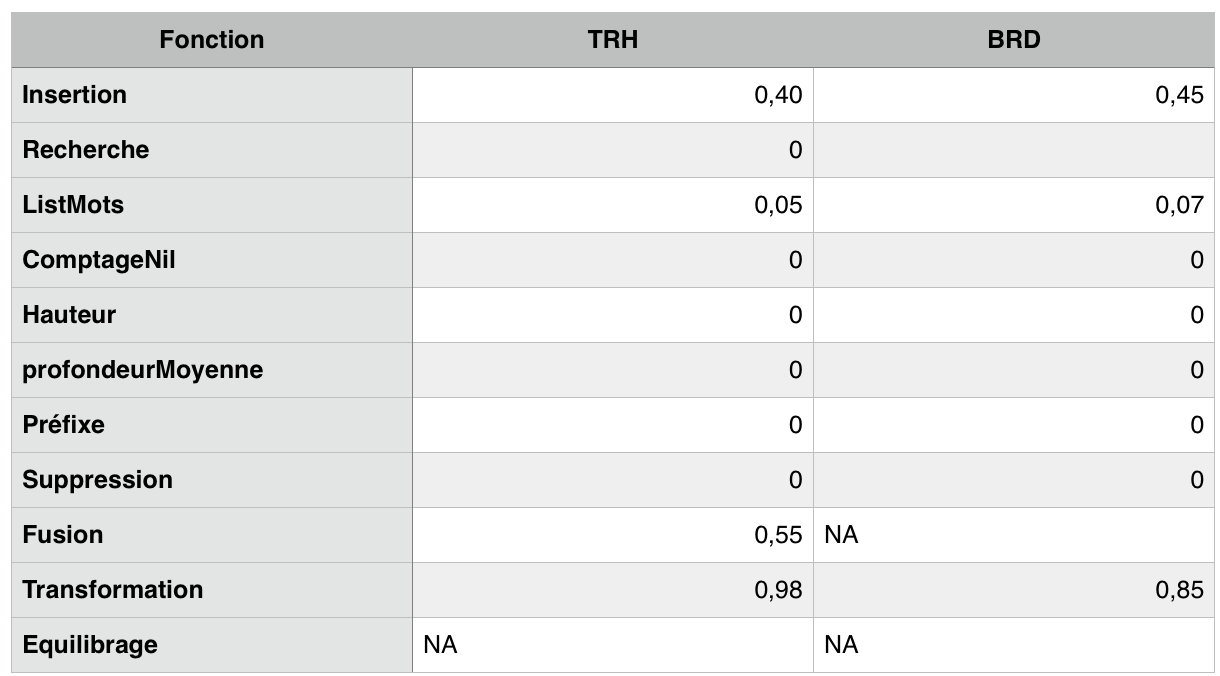
\includegraphics[width=1.0\textwidth]{temps.png}
  \caption{Apercu TRH}
  \label{fig:Aprecu TRH}
\end{figure}

\clearpage
\section*{Affichage visuel en SVG : BRD}\label{sec:name}
\addcontentsline{toc}{section}{Affichage visuel en SVG : BRD}
Vu que graphiz n'est pas du tout adapté au Briandais, on a pris la décision de déssiner nous même l'arbre, sous forme de noeuds en SVG.\\
La librairie de production du format SVG est définie dans src/BRD\_SVGView.c, et comporte notamment la fonction :
void BRDexportToSvgFile(BRDtree* tree, char* filename); qui produit un .svg à partir d'un arbre. Le dessin se fait par facteurs de décallage renvoyés à chaque fois par les fils ...\\
un make run\_unit\_test\_1 produit automatiquement le fichier svg/BRD.svg, qui peut être affiché par un navigateur. ( Sur des gros arbres il est conseillé d'utiliser inkscape, à lancer avec make BRDview )\\
Voici un aperçu de l'exemple de base :\\
\begin{figure}[H]
  \centering
  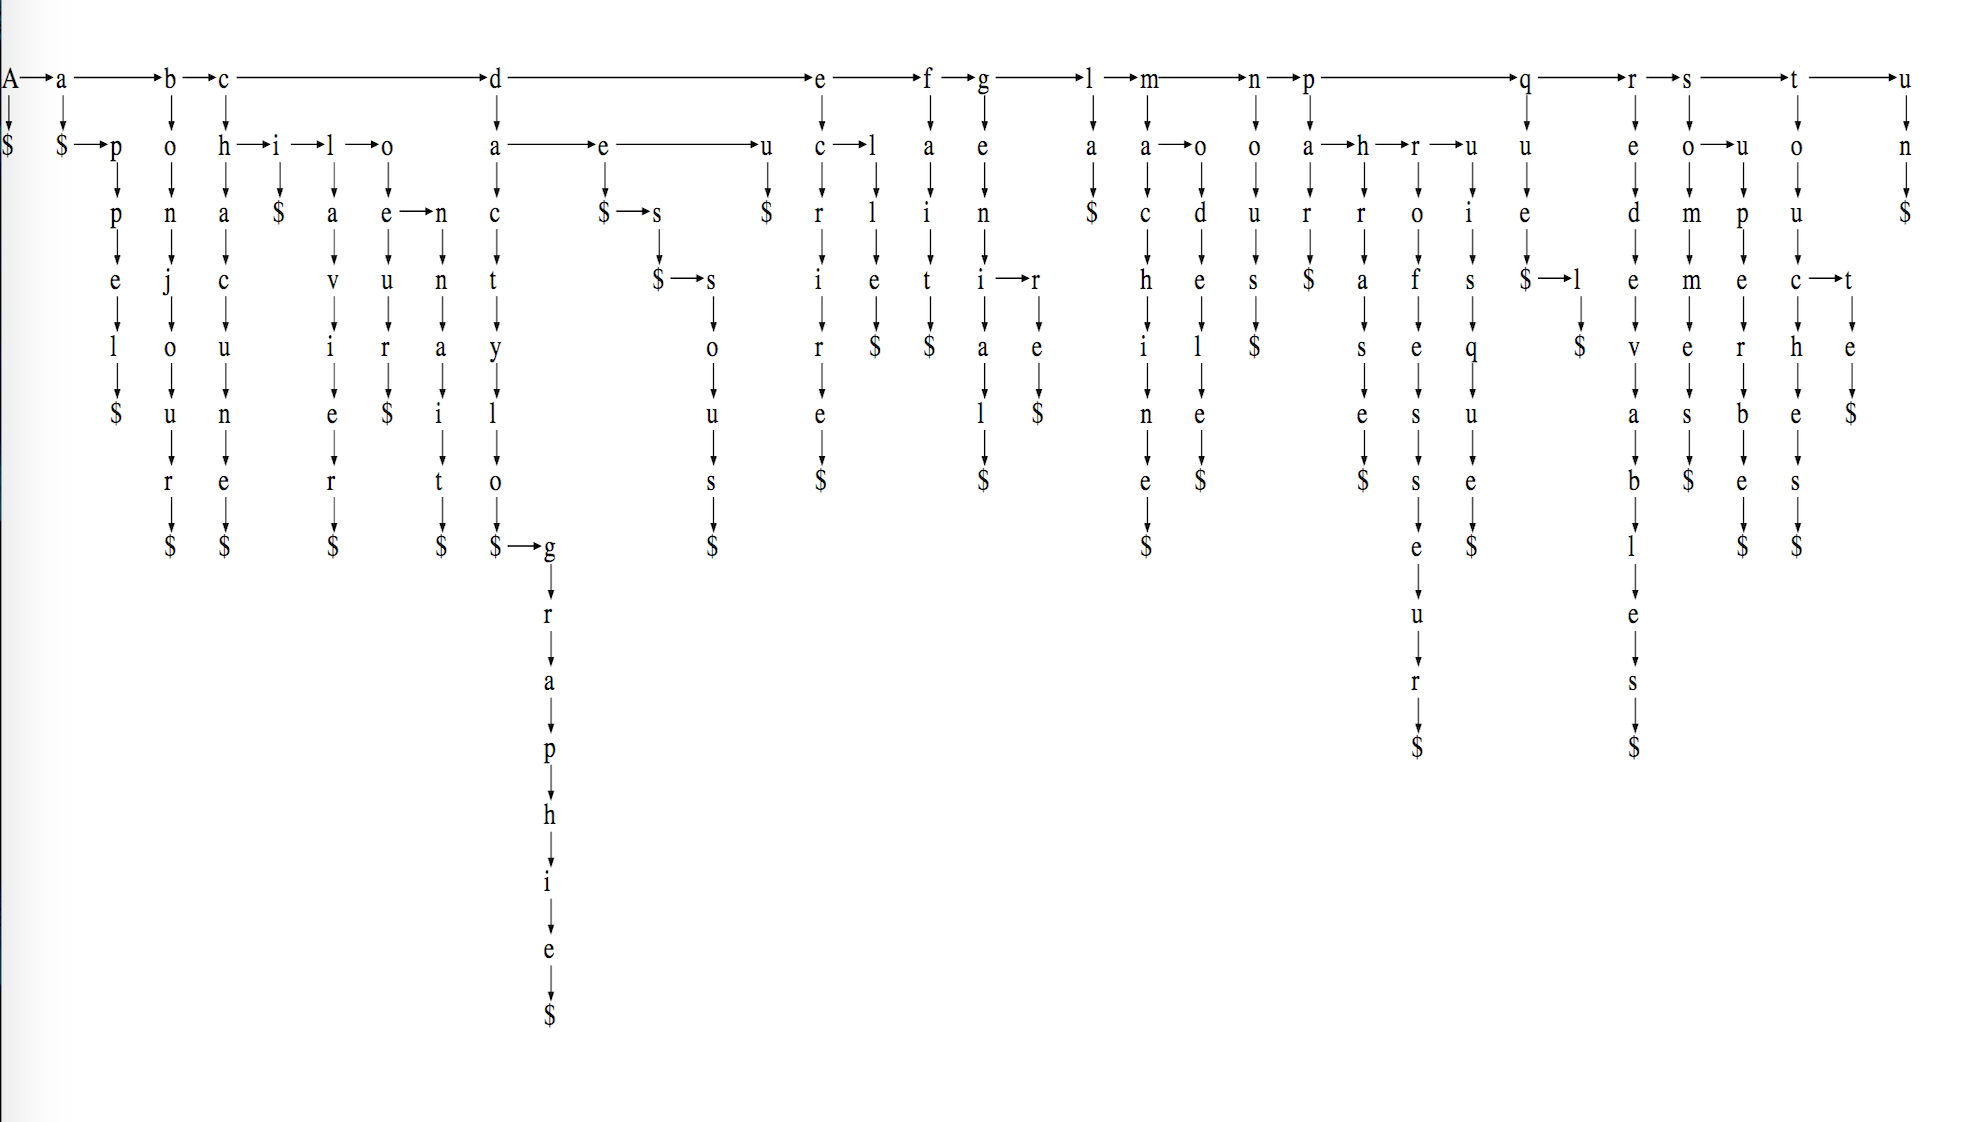
\includegraphics[width=1.3\textwidth]{BRD.png}
  \caption{Apercu BRD}
  \label{fig:Aprecu BRD}
\end{figure}

\clearpage
\section*{Affichage visuel en SVG : TRH}\label{sec:name}
\addcontentsline{toc}{section}{Affichage visuel en SVG : TRH}
Pour l'Hybride on a choisit de faire plus pratique est d'utiliser graphiz.\\
La Lib de production du DOT est définie dans src/TRH\_View.c, et comporte notamment la fonction : \\
void TRHexportToDOTFile(TRHtree* tree);\\
pour transformer le DOT généré en SVG il suffit de faire un make TRHView.\\
Voici un aperçu de l'exemple de base :\\
\begin{figure}[H]
  \centering
  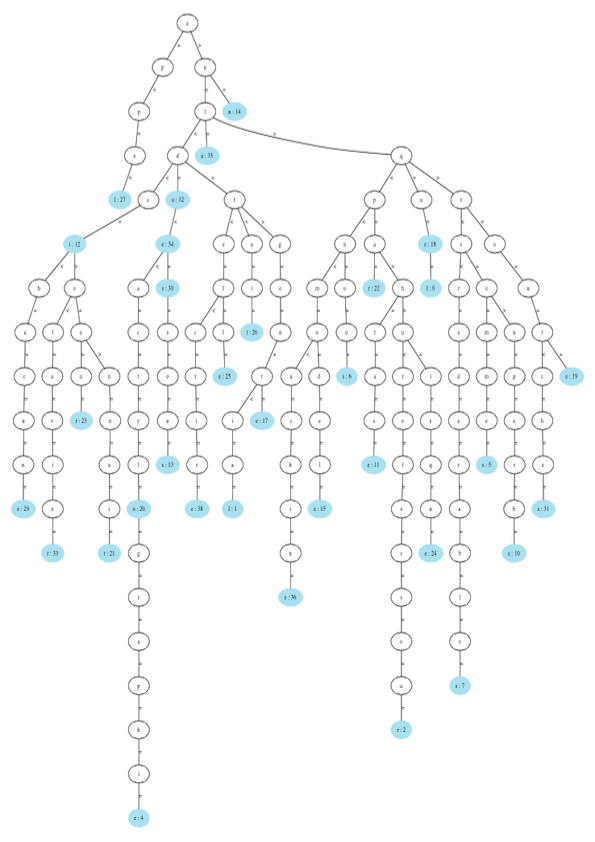
\includegraphics[width=1.0\textwidth]{TRH.png}
  \caption{Apercu TRH}
  \label{fig:Aprecu TRH}
\end{figure}


\end{document}
